

\documentclass[english,11pt]{beamer}

\DeclareMathOperator{\Cov}{Cov}
\DeclareMathOperator{\Var}{Var}
\DeclareMathOperator{\E}{\mathbb{E}}
\DeclareMathOperator{\Proba}{\mathbb{P}}

\newcommand{\Covb}[2]{\ensuremath{\Cov\!\left[#1,#2\right]}}
\newcommand{\Eb}[1]{\ensuremath{\E\!\left[#1\right]}}
\newcommand{\Pb}[1]{\ensuremath{\Proba\!\left[#1\right]}}
\newcommand{\Varb}[1]{\ensuremath{\Var\!\left[#1\right]}}

% norm
\newcommand{\norm}[1]{\| #1 \|}

\newcommand{\indep}{\rotatebox[origin=c]{90}{$\models$}}





\usepackage{mathptmx,amsmath,amssymb,graphicx,bibentry,bbm,babel,ragged2e}

\makeatletter

\newcommand{\noun}[1]{\textsc{#1}}
\newcommand{\jitem}[1]{\item \begin{justify} #1 \end{justify} \vfill{}}
\newcommand{\sframe}[2]{\frame{\frametitle{#1} #2}}

\newenvironment{centercolumns}{\begin{columns}[c]}{\end{columns}}
%\newenvironment{jitem}{\begin{justify}\begin{itemize}}{\end{itemize}\end{justify}}

\usetheme{Warsaw}
\setbeamertemplate{footline}[text line]{}
\setbeamertemplate{headline}{}
\setbeamercolor{structure}{fg=purple!50!blue, bg=purple!50!blue}

\setbeamersize{text margin left=15pt,text margin right=15pt}

\setbeamercovered{transparent}


\@ifundefined{showcaptionsetup}{}{%
 \PassOptionsToPackage{caption=false}{subfig}}
\usepackage{subfig}

\usepackage[utf8]{inputenc}
\usepackage[T1]{fontenc}

\usepackage{multirow}

\usepackage{mdframed}


%\AtBeginSection[]
%{
%  \begin{frame}
%  \frametitle{}
%  \tableofcontents[currentsection]
%  \end{frame}
%}

\makeatother




\begin{document}

\title[Agent-based modeling city networks]{An agent-based model for city networks based on interactions between firms}
\author[Raimbault \and Zdanowska]{J.~Raimbault$^{1,2,3\ast}$ \and N. Zdanowska$^{1,3}$\\\medskip
$^{\ast}$\texttt{j.raimbault@ucl.ac.uk}
}

\institute[UCL]{$^{1}$CASA, UCL\\
$^{2}$UPS CNRS 3611 Complex Systems Institute Paris\\
$^{3}$UMR CNRS 8504 G{\'e}ographie-cit{\'e}s
}


\date[2nd October 2019]{CCS 2019\\
Satellite Simulation models\\
October 2nd 2019
}

\frame{\maketitle}

\section{Introduction}


\sframe{Urban firm networks}{

Cities as maximisation of socio-economic interactions 


Network economies \cite{sassen1991global} \cite{castells1996information}

World city network driven by interactions between firms \cite{taylor2001specification} \cite{martinus2018global}

Asymmetrical spatial interactions -- different relative position of cities

}


\sframe{An evolutionary approach to Urban Systems}{

Evolutionary Theory of Urban Systems \cite{pumain1997pour} \cite{pumain2006villes}

Adaptive cycles and diffusion on innovation (H{\"a}gerstrand, 1973)

Path dependence

Selection

Emergent structures


}

\sframe{Firm linkages structuring urban systems}{

% examples de resultats pour l'Europe Centrale et Orientale




 \begin{center}
 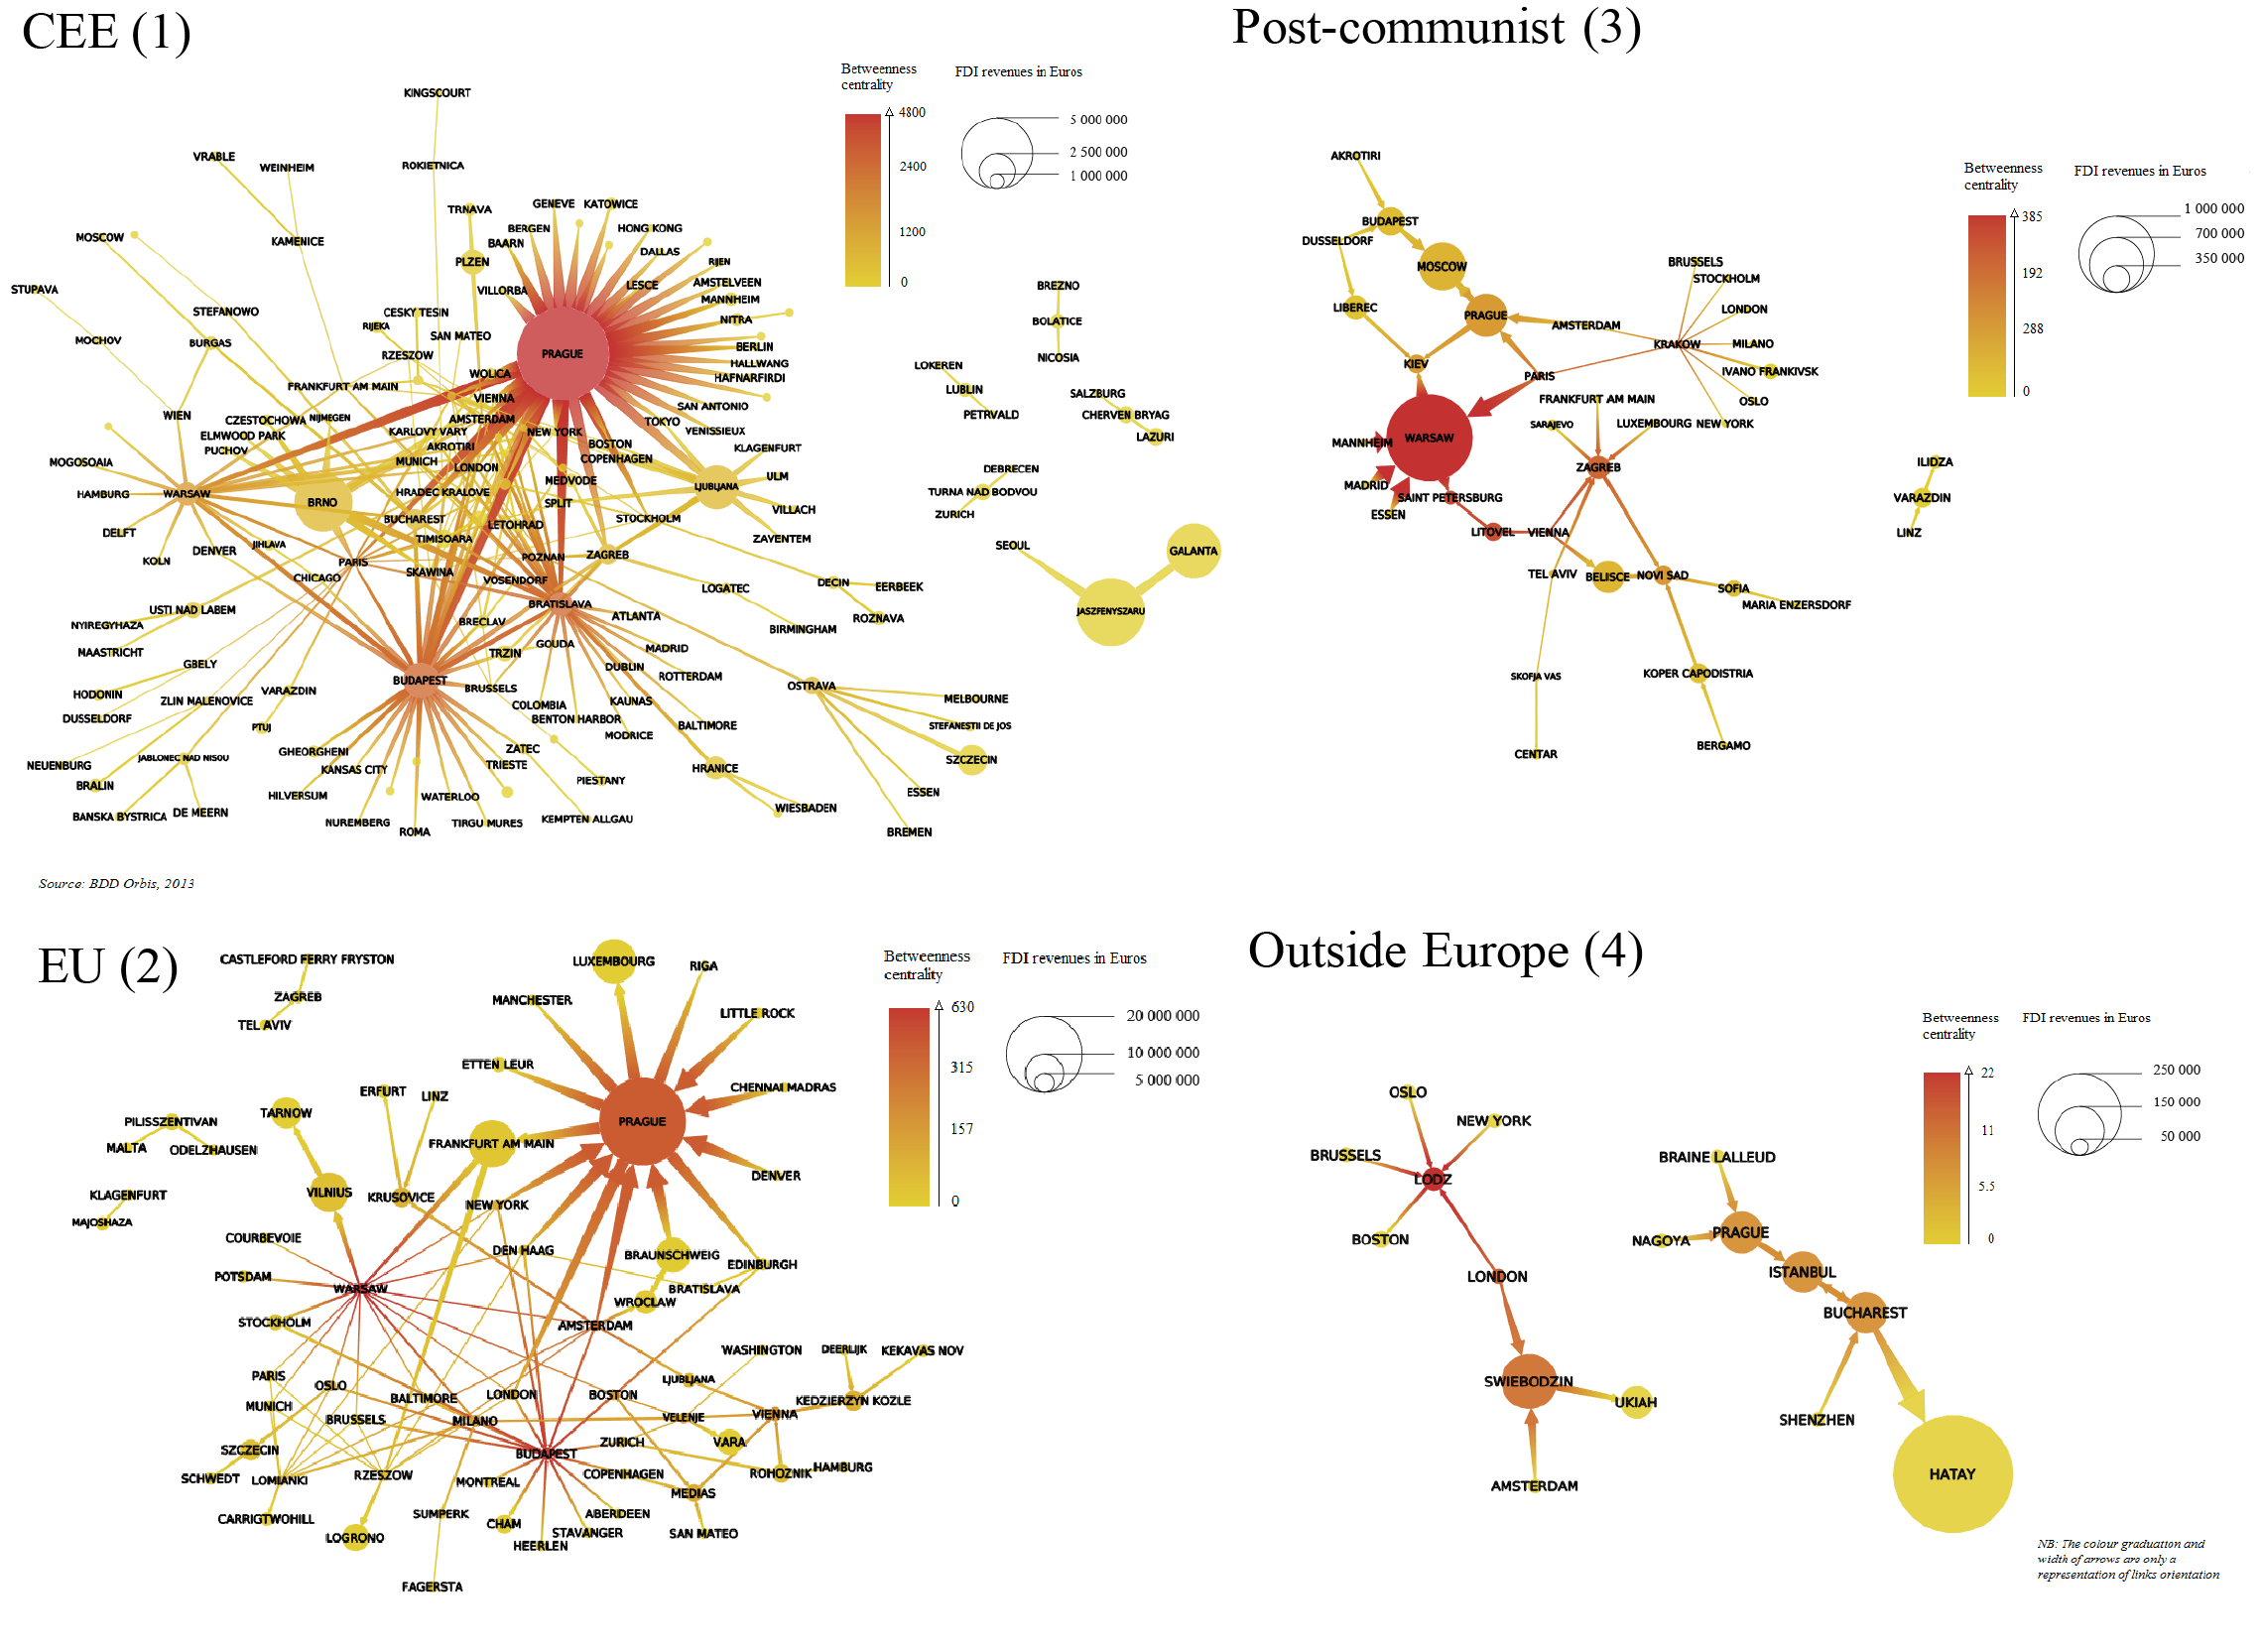
\includegraphics[width=0.7\textwidth]{figures/Figure1.png}
 \end{center}
 
  \textit{Central and Eastern European cities within ownership links of firms in 2013.}

}

% si besoin je peux rajouter d'autres exemples sur le UK ou carrement des trucs de Celine sur les reseaux de firmes

\sframe{Urban Firm linkages and geo-economic processes}{

Metropolisation vs. regionalisation effects

Relationship local/global of multinational firm linkages (internationalisation)

Specialisation-driven factors for an economic network to emerge

Drivers of innovation

Macroeconomic exogenous chocs and resilience of urban systems

Can we access geographical and economic processes within urban networks of firms with a generative model? 

}
\sframe{Towards a generative model of urban firm networks}{

% research question / objective
% du coup je te laisse formuler le broad research question, car je vois pas bien


}

\section{Model}

\sframe{Model rationale}{

}


\sframe{Formalization}{

Cities characterized by economic size $E_i$ (GDP) and economic structure $s_{ik}$

\bigskip

Starting from an initial network, at each time step:
\begin{enumerate}
    \item Evolve cities with an interaction model (\cite{raimbault2018indirect} or \cite{cottineau2015growing})
    \item Add a fixed number of links randomly, following a probability function of sizes, sector proximity, and geographical and socio-cultural proximities
\end{enumerate}

}


\sframe{Formalization}{

Probability for a new link follows a generalized Cobb-Douglas function

\begin{equation}
     p_{ij} \propto \left(\frac{E_{i}}{E}\right)^{\gamma_F} \cdot \left(\frac{E_{j}}{E}\right)^{\gamma_T} \cdot \left(\frac{w_{ij}}{W}\right)^{\gamma_W} \cdot s\left(S_{ik},S_{jk}\right)^{\gamma_S} \cdot \exp \left(- \gamma_D \cdot d_{ij}\right) \cdot \exp \left(- \gamma_G \cdot g_{ij}\right)
\end{equation}

}

\sframe{Model indicators}{

Geographical indicators:

\begin{itemize}
    \item Internationalisation
    \item Metropolisation
    \item Regionalisation
    \item Specialisation
\end{itemize}

\bigskip

Network and flows indicators

}

\sframe{Simulation on synthetic systems of cities}{

% la ou avant il faut surement expliquer que c'est pas totalement synthetique, que tu pars de X villes europeennes de plus de 50 000 habitants (pour les plus nuls comme moi)
% si c'est completement synthetiques, l'histoire des villes europeenes c'est pour avoir les ordres de grandeur de la hierarchie et du nombre de villes, mais c'est pas parametrise sur des vraies donnees - mais oui ca ca sera explique dans comment construire le systeme de ville synthetique.
 
\textit{Following \cite{raimbault2018space}, geosimulation models must be studied within synthetic controllable urban contexts (spatial sensitivity)}

\bigskip



 
}

\section{Results}

\sframe{Implementation}{

% for now no dynamics of cities

\begin{itemize}
	\item Model implemented in NetLogo (good compromise interactivity / ergonomy), with fast data structures (matrix/table extensions)
	\item Integrated into OpenMOLE \cite{reuillon2013openmole} for model exploration
	\item Current implementation: only network dynamics 
\end{itemize}

}

\sframe{Simulation of urban networks}{
    
    % examples
    
    \centering
    
    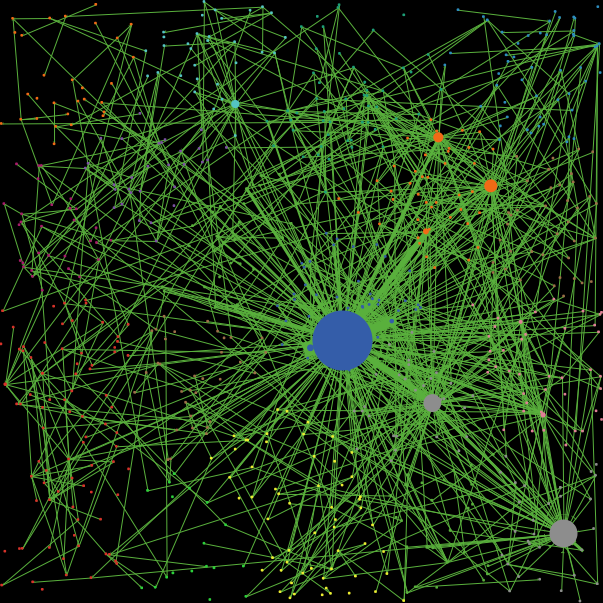
\includegraphics[width=0.48\textwidth]{figures/ex_alleq-highgravity_seed-12102_t1500.png}\hspace{0.1cm}
    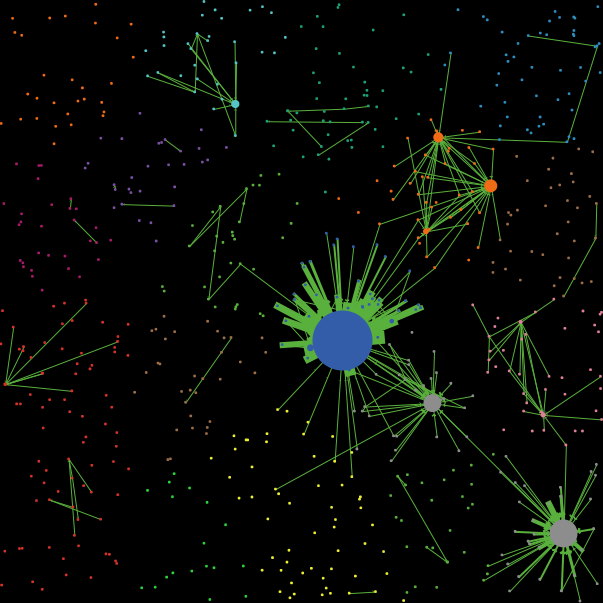
\includegraphics[width=0.48\textwidth]{figures/ex_alleq-lowgravity_seed-12102_t1500.png}

	\medskip

	\textit{Networks at $t=1500$, for default parameters values and high gravity (left) and low gravity (right)}

}


\sframe{Statistical convergence}{

$\rightarrow$ Good convergence for most indicators: average sharpes ratios on a one-factor sampling above 5 (except for metropolization index $\simeq 1.5$)

% + histograms

\bigskip




}


\sframe{Interaction decay}{
    
    % One factor sampling results
    %  20190924_162740_ONEFACTOR_REPLICATIONS_SYNTHETIC_GRID
    
    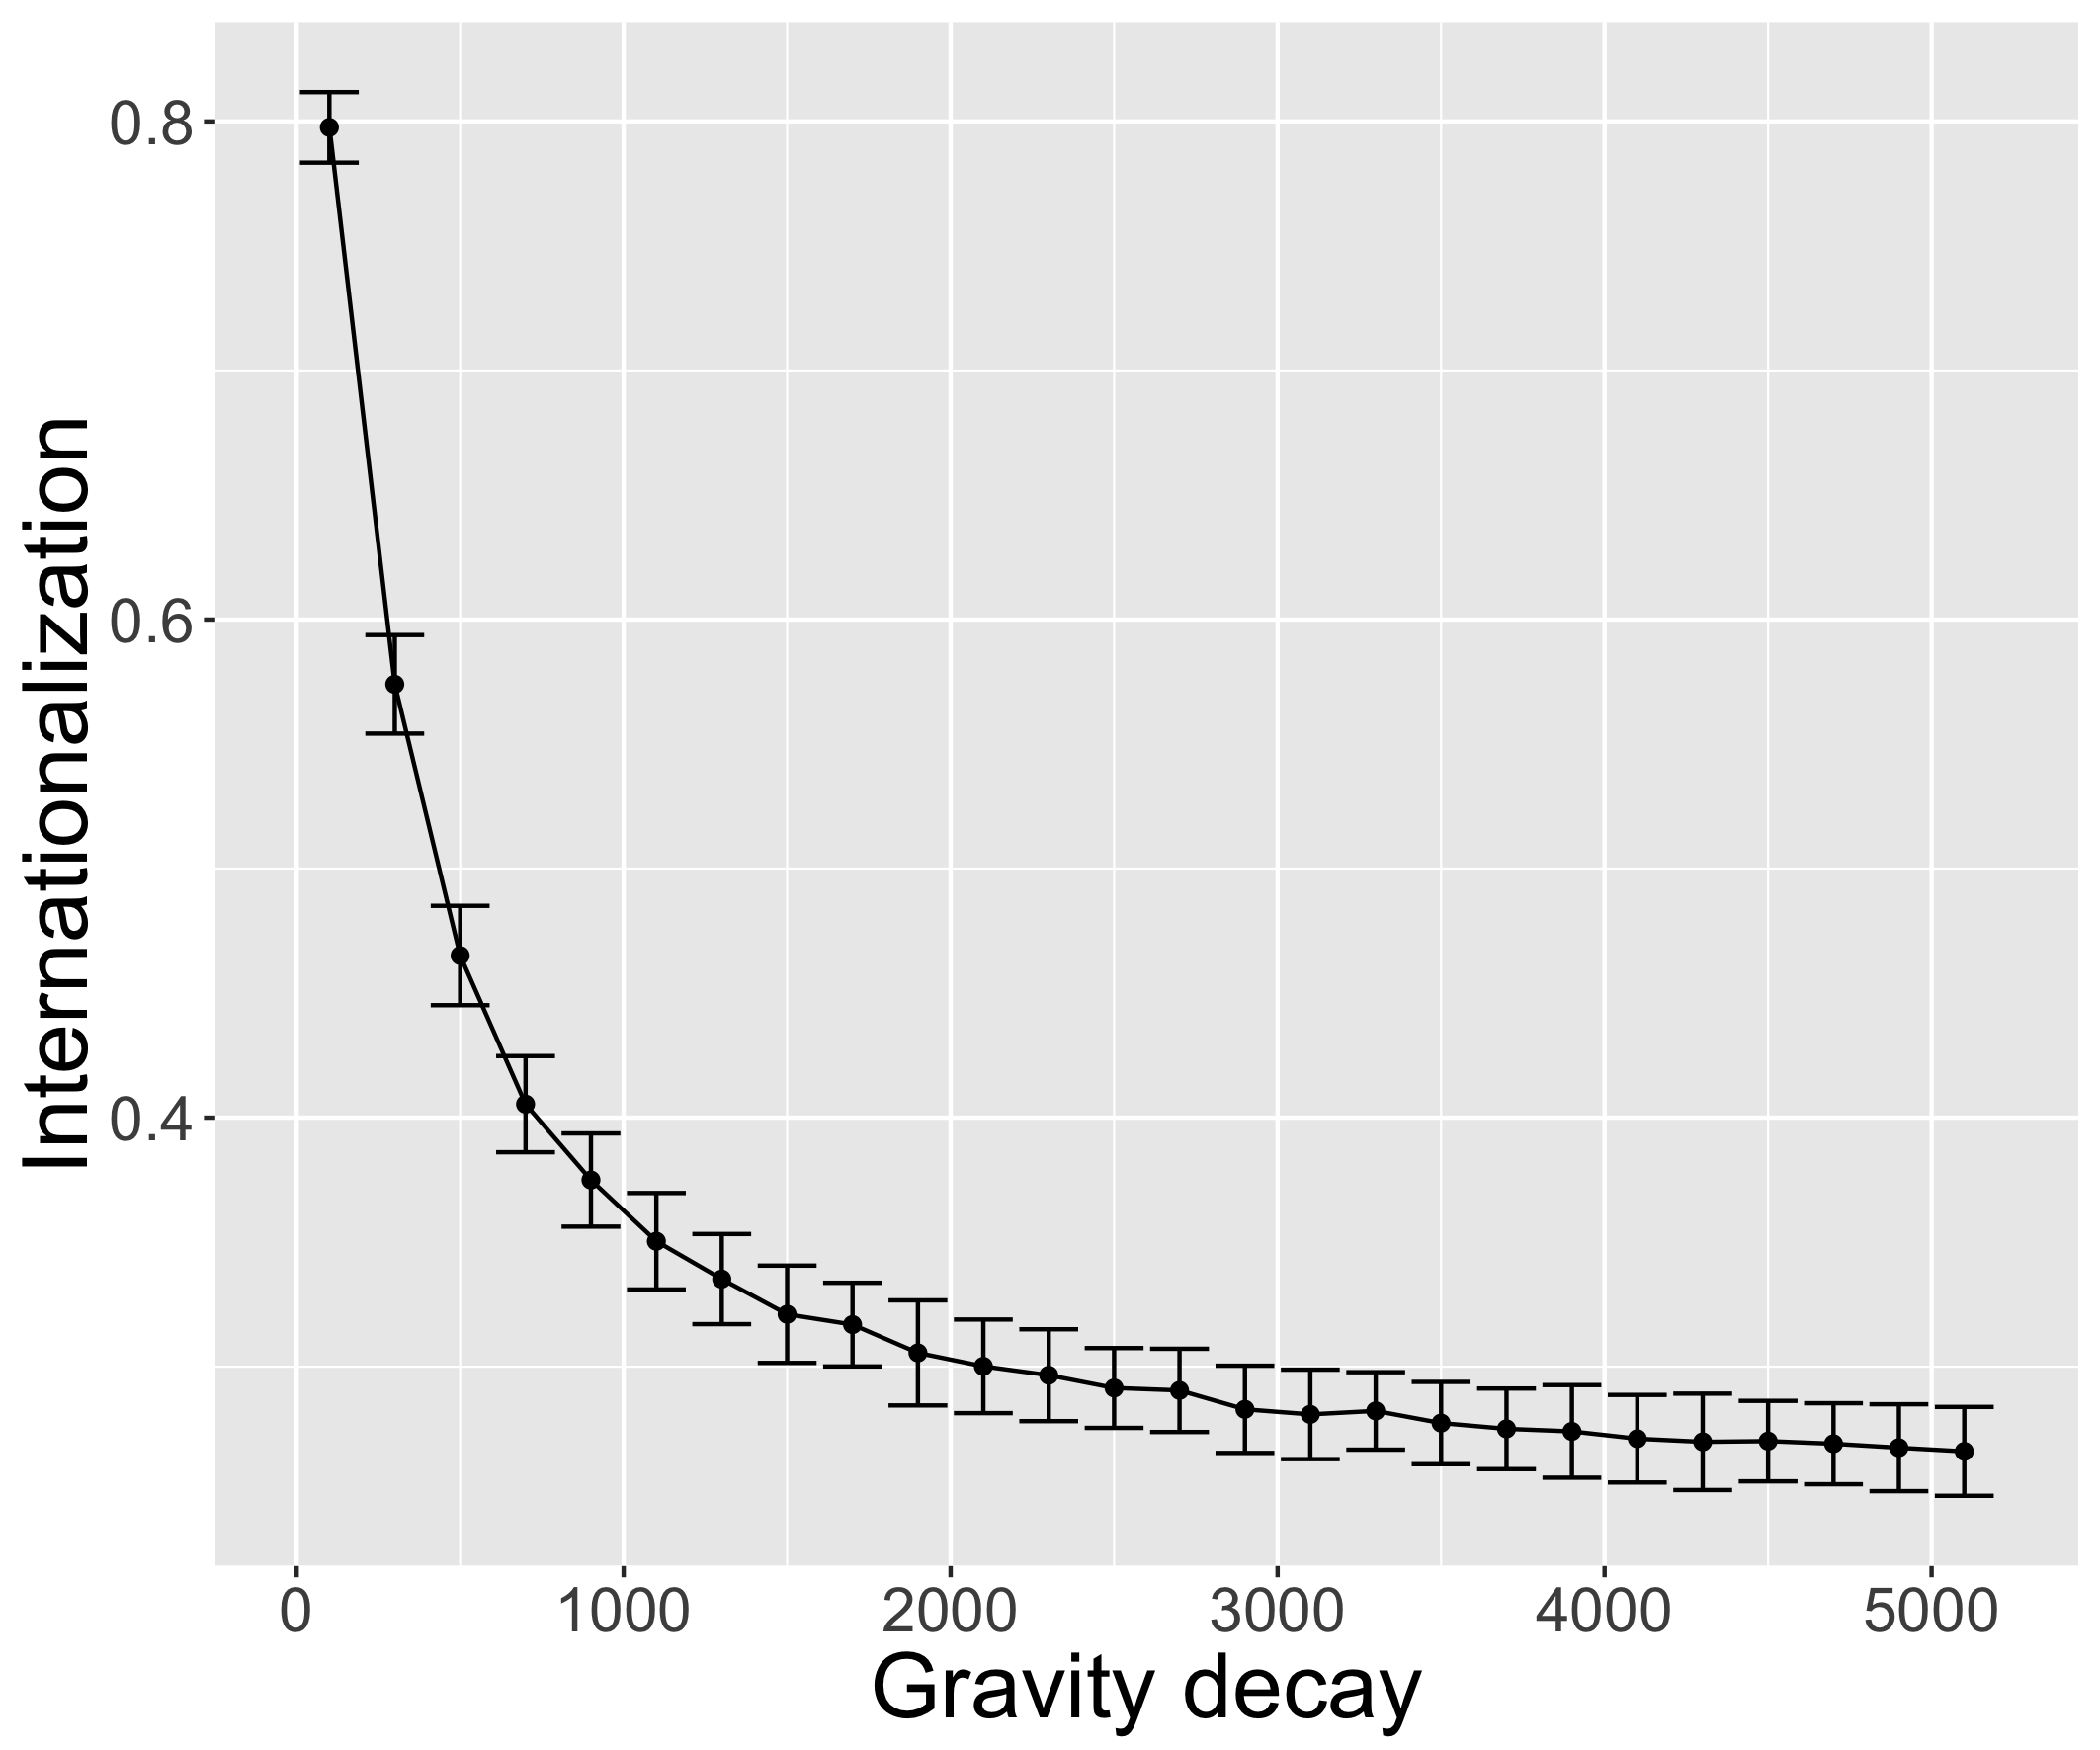
\includegraphics[width=0.48\textwidth]{figures/internationalization-gravityDecay_errorbars.png}
    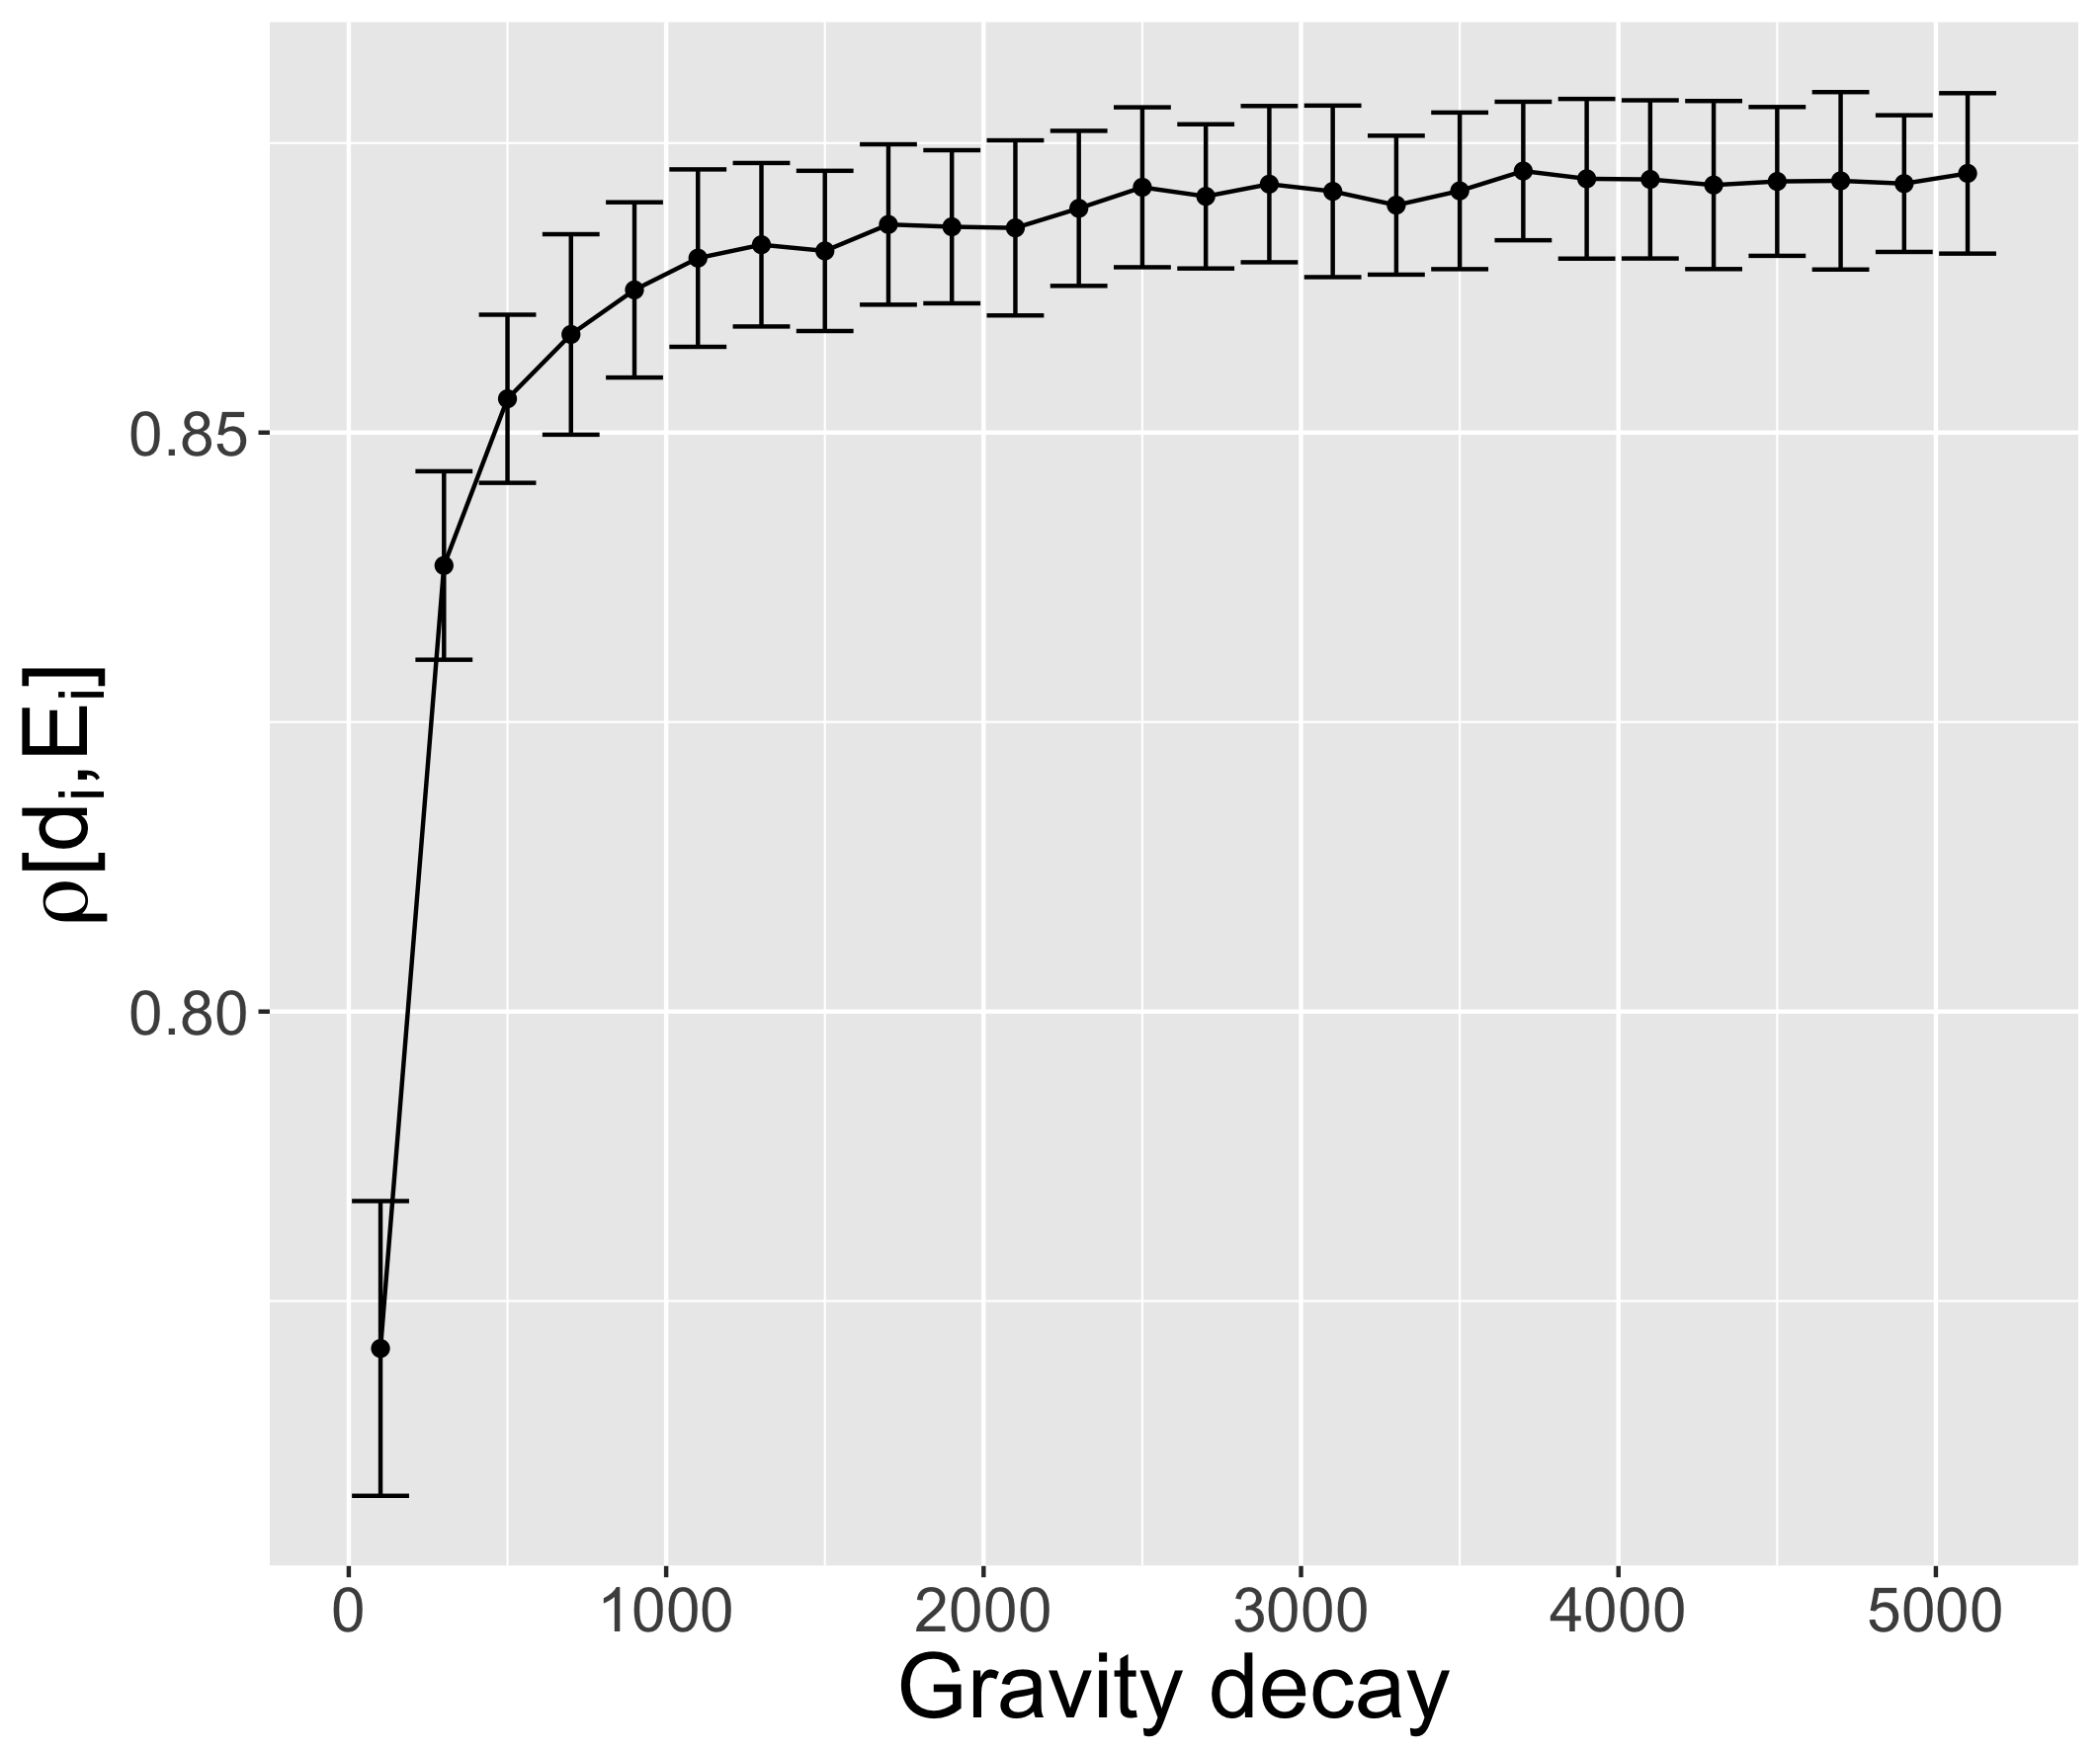
\includegraphics[width=0.48\textwidth]{figures/rhoDegreeSize-gravityDecay_errorbars.png}
}

\sframe{Sector proximity}{
    
    % One factor sampling results
    %  20190924_162740_ONEFACTOR_REPLICATIONS_SYNTHETIC_GRID
    
     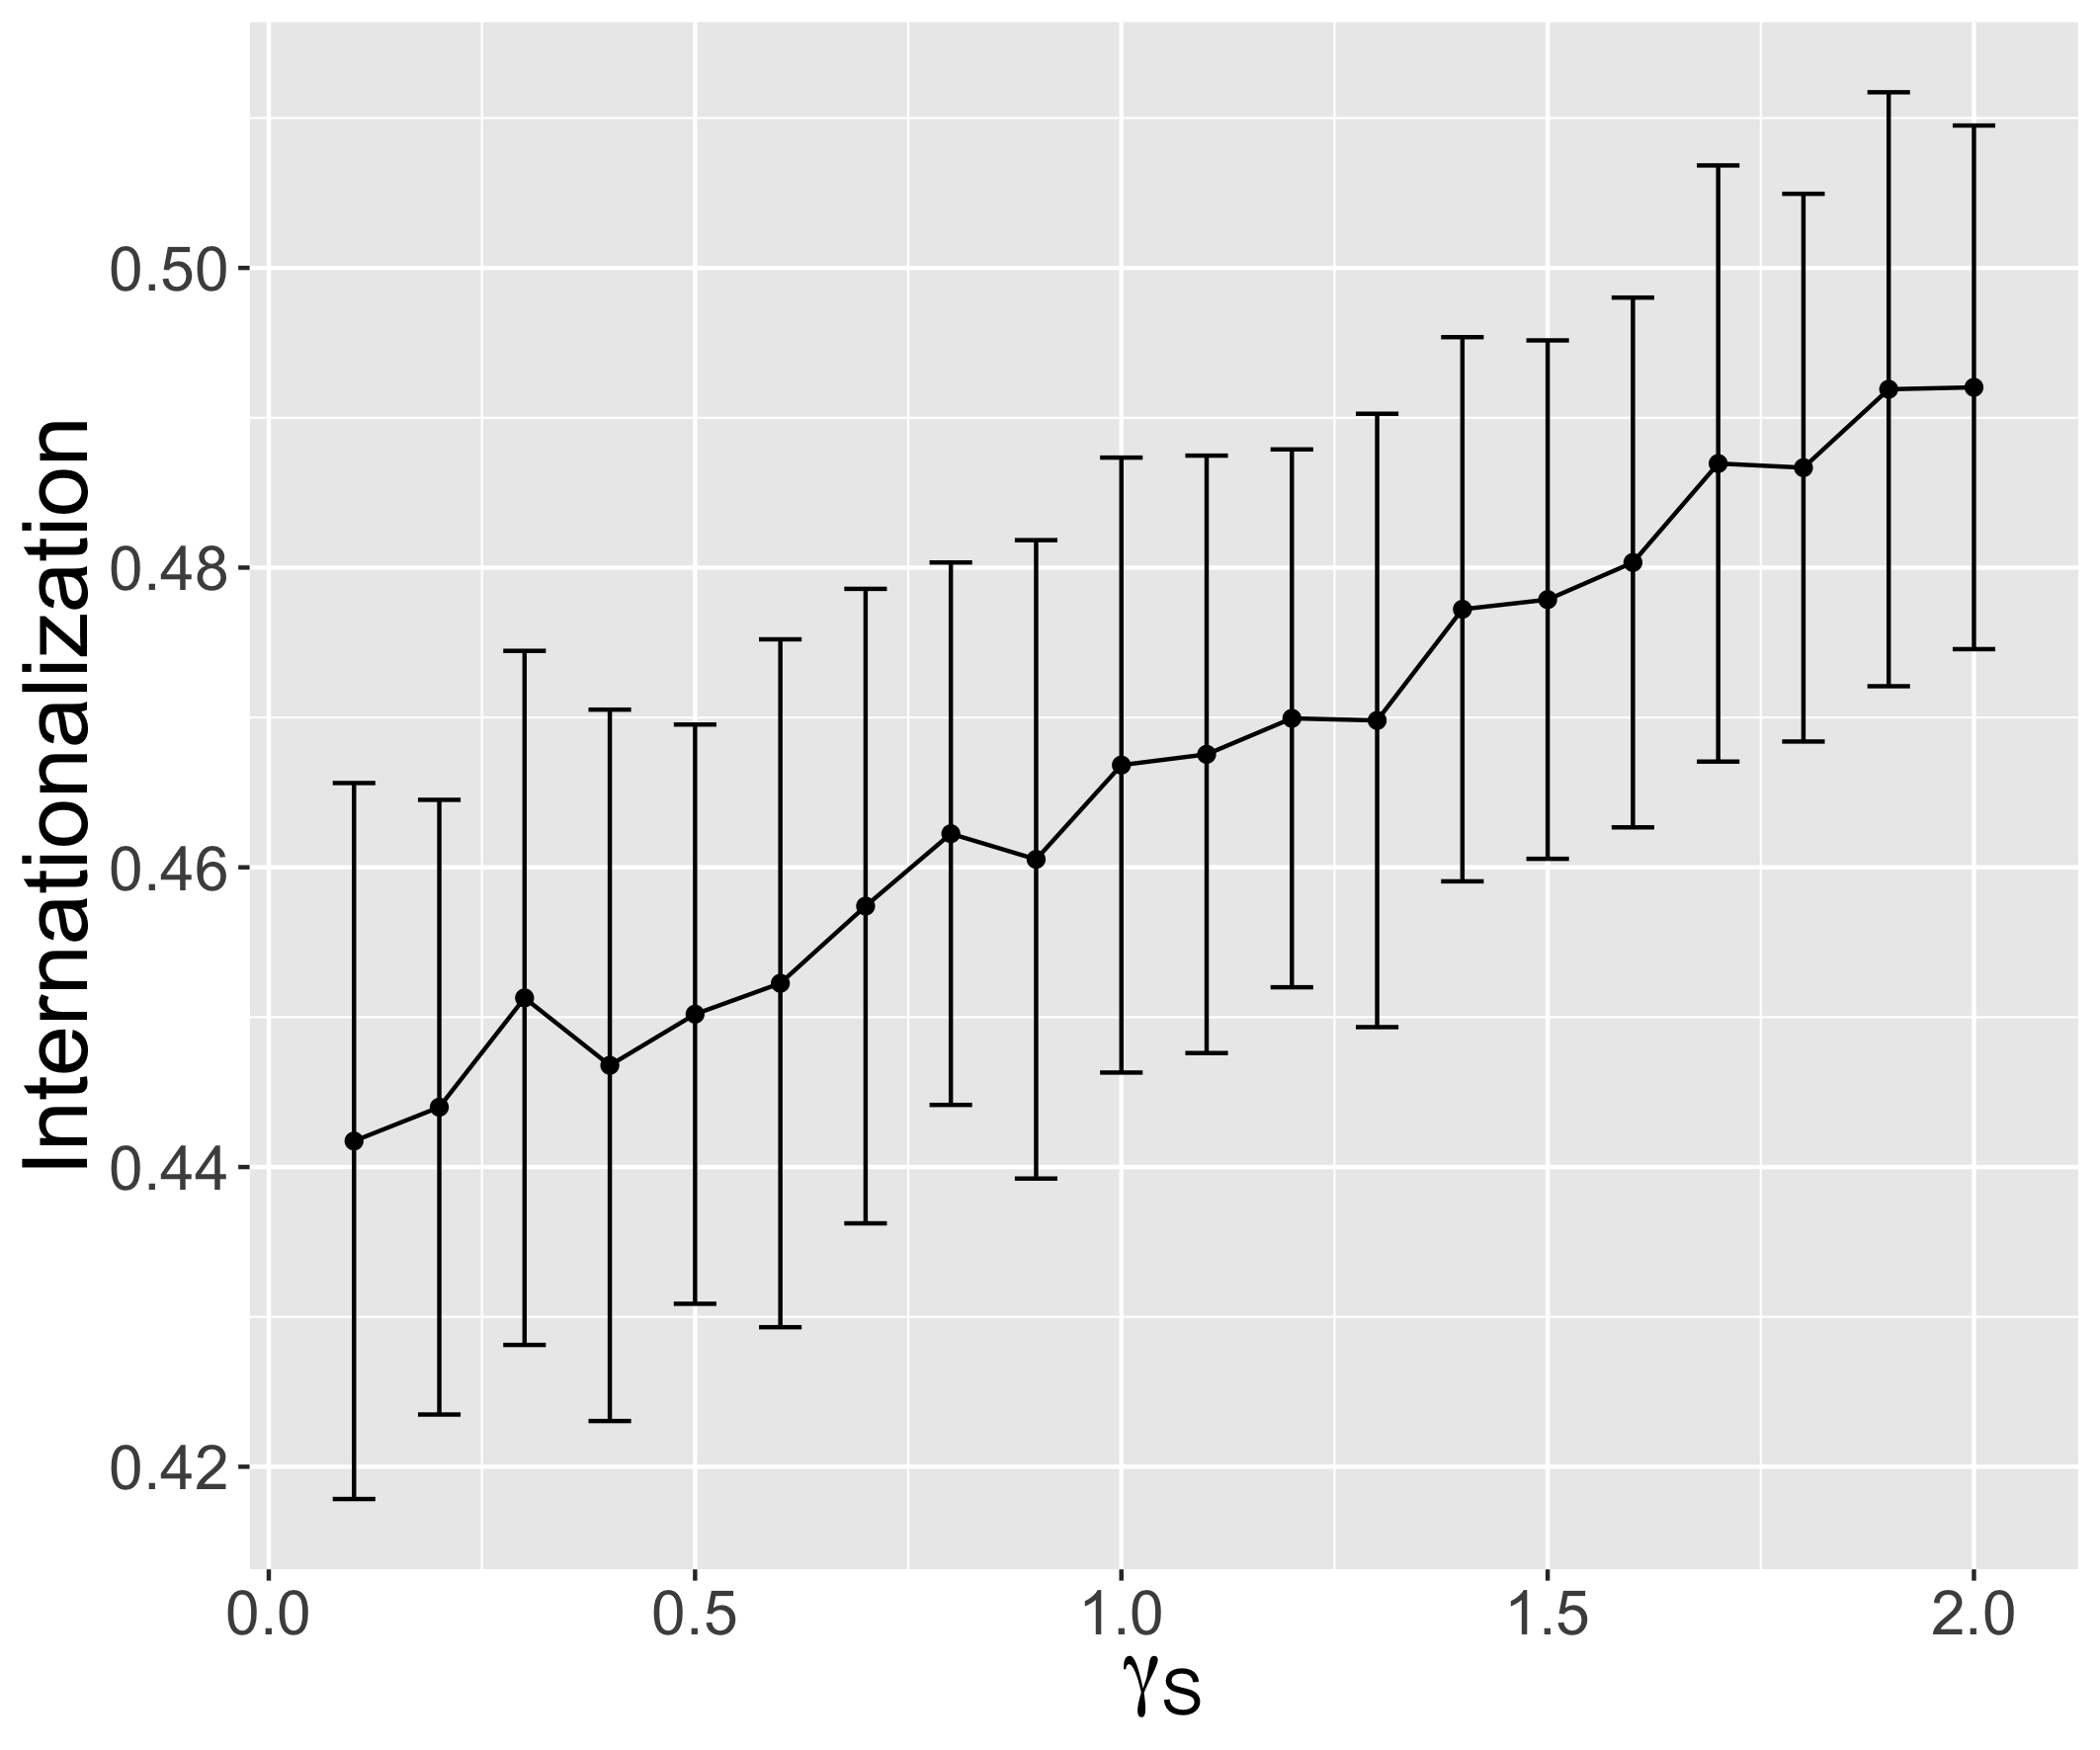
\includegraphics[width=0.48\textwidth]{figures/internationalization-gammaSectors_errorbars.png}
    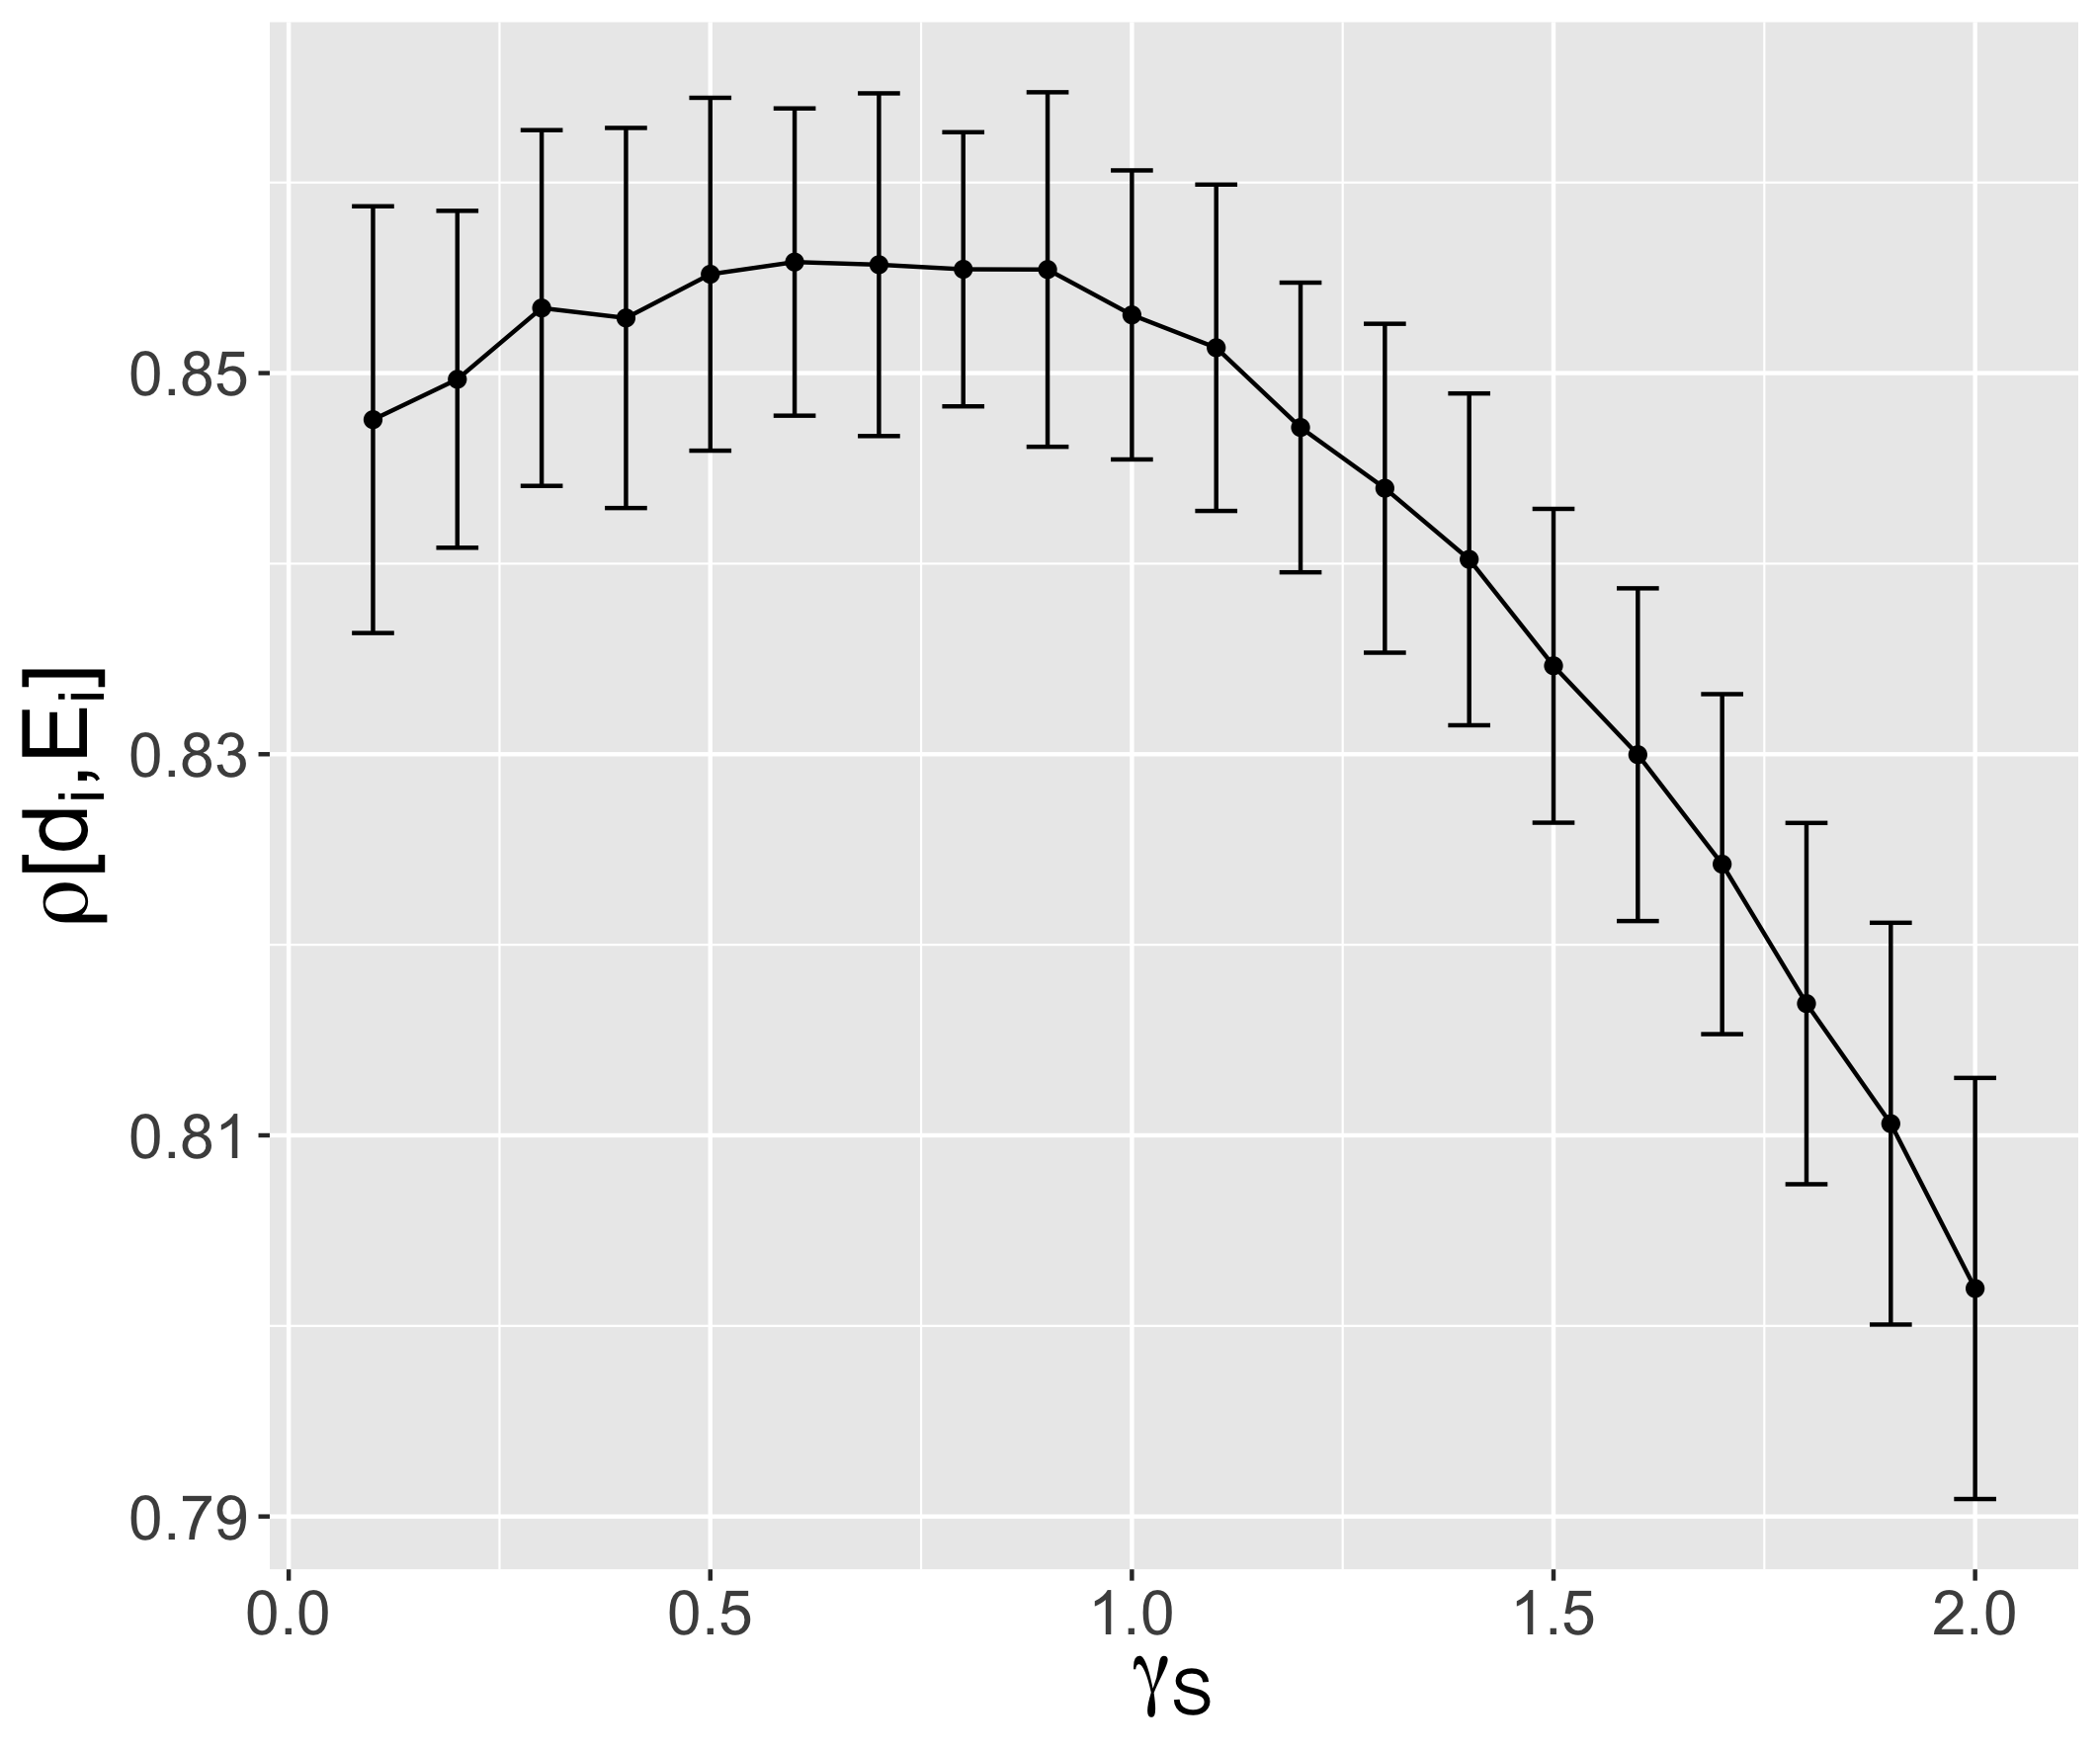
\includegraphics[width=0.48\textwidth]{figures/rhoDegreeSize-gammaSectors_errorbars.png}
    
    
}

\sframe{Grid exploration}{

}

% other experiments ? PSE on correlations ?




\section{Discussion}

% - future work etc (classical discussion)
% - on the role of model exploration and simulation to gain knowledge from the model

% comparing with real data?

\sframe{On the role of model exploration}{

}


\sframe{Discussion}{

\textbf{Practical application}



\textbf{Developments}


}


\sframe{Conclusion}{

$\rightarrow$ A simulation model to understand processes of network emergence

$\rightarrow$ 


\bigskip
\bigskip


\textbf{Open repository for model and results at}

\texttt{https://github.com/JusteRaimbault/ABMCitiesFirms}

\textbf{Simulation data at}

\texttt{}% dataverse

\bigskip

\textbf{Acknowledgments}: thanks to the \textit{European Grid Infrastructure} for access to the infrastructure.


}



\sframe{Reserve slides}{

\centering

\Large

\textbf{Reserve Slides}

}



%%%%%%%%%%%%%%%%%%%%%
\begin{frame}[allowframebreaks]
\frametitle{References}
\bibliographystyle{apalike}
\bibliography{biblio}
\end{frame}
%%%%%%%%%%%%%%%%%%%%%%%%%%%%







\end{document}

